\documentclass[envcountsect]{llncs}
\bibliographystyle{splncs04}
\pagestyle{headings}

% = = = = = Packages = = = = = %

% !TEX root = ../main.tex

%------------------------LNCS----------------------%

%None

%------------------------Packages----------------------%

% = = = Graphics
\usepackage[pdftex]{graphicx}
\graphicspath{{figures/}}
\DeclareGraphicsExtensions{.jpg,.png}
\usepackage[table,xcdraw]{xcolor}

% = = = Subfig (note not subfigure)
\usepackage[caption=false,font=footnotesize]{subfig}

% = = = Math Symbols
\usepackage{amsmath}
%\usepackage{amstext,amssymb,amsthm}
\usepackage{bbm}
\usepackage{stmaryrd}

% = = = Other
\usepackage{array}
\usepackage{color}
\usepackage[hyphens]{url}
\usepackage[pdftitle=Title,pdfauthor=Anonymous]{hyperref}

%------------------------END----------------------%  
  


% !TEX root = ../main.tex
%------------------------Custom Commands----------------------%

% = = = Latin Short-forms (ie, eg, etc, et al)
\usepackage{xspace}
\newcommand{\etal}{\textit{et al.}\xspace}
\newcommand{\etc}{\textit{etc.}\xspace}
\newcommand{\ie}{\textit{i.e.,}\xspace}
\newcommand{\eg}{\textit{e.g.,}\xspace}
\newcommand{\cf}{\textit{cf.}\xspace}
\newcommand{\supra}{\textit{Supra}\xspace}
\newcommand{\nee}{\textit{n\'ee}\xspace}


% = = = Arrow -> (\lt)
\newcommand{\lt}{$\rightarrow$\xspace}

% = = = Keywords (kw)
\newcommand{\kw}[1]{\textsf{#1}}

% = = = Colored text (textblue)
\newcommand{\textblue}[1]{\textcolor{blue}{#1}}

% = = = Compact Lists (compactlist, compactlistn)
\newenvironment{compactlist}
  {\begin{itemize} 
  \setlength{\itemsep}{0pt} 
  \setlength{\parskip}{0pt}} 
  {\end{itemize}}
  
\newenvironment{compactlistn}
  {\begin{enumerate} 
  \setlength{\itemsep}{0pt} 
  \setlength{\parskip}{0pt}} 
  {\end{enumerate}}
  
\renewcommand{\labelitemi}{$\bullet$}
  

%------------------------Crypto----------------------%  

% = = = Zp, Gq and Zq
\newcommand{\Zp}{\mathbb{Z}^{*}_{p}}
\newcommand{\Zq}{\mathbb{Z}_{q}}
\newcommand{\Gq}{\mathbb{G}_{q}}

% = = = Encryption, etc.
\newcommand{\Enc}[1]{\mathsf{Enc}(#1)}
\newcommand{\EncB}[1]{\llbracket #1 \rrbracket}
\newcommand{\ReRand}[1]{\mathsf{ReRand}(#1)}
\newcommand{\Hash}[1]{\mathcal{H}(#1)}
\newcommand{\Sign}[1]{\mathsf{Sig}(#1)}
\newcommand{\Comm}[1]{\mathsf{Comm}(#1)}
\newcommand{\Open}[1]{\mathsf{Open}(#1)}

% = = = Tuples
\newcommand{\tuple}[1]{\left \langle #1 \right \rangle}


%-------------------Custom for Paper----------------------%

% = = = Name
\newcommand{\Name}{\textsf{System Name}\xspace}






% !TEX root = ../main.tex

% = = = Rotated Table Entry \headrow

\usepackage{adjustbox}
\newcommand{\headrow}[1]{\multicolumn{1}{c}{\adjustbox{angle=45,lap=\width-0.5em}{#1}}}

% = = = Table bullets: \full and \prt (full and part)

\newcommand{\full}{$\bullet$}
\newcommand{\prt}{$\circ$}






%\usepackage[all=normal,floats=tight,paragraphs=tight]{savetrees}

% = = = = = Title = = = = = %

\begin{document}
\frontmatter
\mainmatter

\title{\Large \bf Short Paper: Red-Black Coins}

%\author{Mehdi Salehi \and Jeremy Clark \and Mohammad Mannan}
%\institute{Concordia University}

\maketitle


% = = = = = Abstract = = = = = %

% !TEX root = ../main.tex
\begin{abstract}

Abstract goes here. 

\end{abstract}

% = = = = = Main Body = = = = = %

% !TEX root = ../main.tex

% = = = = = = = = = = = = = = = = = = = = = = = = = = = = = = = = = = = = = = = = = =

\section{Introductory Remarks}

Cryptocurrencies like Bitcoin (BTC) and Ether (ETH) are marked by extreme volatility in price relative to the US dollar (USD). As decentralized finance (DeFi) services mature on Ethereum, a critical component to their success is letting users choose between holding ETH and holding a stablecoin that targets USD (or some other metric of stability) in price.

Some stablecoins work like a hypothetical vending machine~\cite{CDM20}: Alice deposits two `coins' from a volatile currency (\eg a cryptocurrency like ETH) into the machine and it returns to her two new coins---a `black' coin that is stable and a `red' coin that is even more volatile in price than the original coins Alice put in. Together, the red and black coins are equal in value to the two input coins. The machine cannot reduce overall price volatility, but it can push volatility from the black coin onto the red coin. 

Consider the following example of such a stability mechanism. An asset is chosen that is considered stable by definition (\eg the US dollar). The vending machine is implemented as a decentralized app (DApp; \aka smart contract) on a blockchain (\eg Ethereum). Alice deposits an amount of ETH worth \$1.50 USD into the DApp. The DApp references a trusted oracle service for the current ETH/USD exchange rate to enforce this. The DApp holds the ETH as a deposit for future redemption, and returns to Alice a red coin and a black coin (\eg as ERC-20 tokens). Alice can sell one or both coins. In the future, the owner of the black coin can redeem it for ETH from the DApp, and receive the equivalent of \$1.00 USD. This assumes the initial deposit of \$1.50 USD worth of ETH is still worth at least \$1.00 USD at redemption time---if not, the black coin owner receives all of the collateral. The red coin holder receives any remaining ETH after the black coin holder is paid.

The key idea is that the black coin will nearly always be worth the equivalent of \$1.00 USD. This is true when ETH/USD increases in value, stays the same, or declines moderately. Only if it declines significantly does the black coin start to experience volatility in price---its redemption value will decrease at the same rate as ETH/USD itself. For the red coin, the redemption value increases and decreases as ETH/USD itself increases and decreases, however the gains and losses are amplified. This is an overview; we return to these details below.

\paragraph{Synthetic Assets.} The red-black coin primitive can be generalized to produce black coins that match the price of any financial asset, not just a currency like the USD, simply by changing the price that the oracle references. For example, a black coin for one share of the company Apple (APPL) would use an ETH/APPL price feed (possibly constructed by bridging ETH/USD and APPL/USD prices) and otherwise be exactly the same. These black coins are `synthetic assets' because they expose the holder to the price movements of the asset but do not afford the holder any other benefits of holding the financial instrument (\eg shareholder votes or dividends for equities; physical delivery for futures; or the ability to settle a loan, or option contract on the asset). What a red coin represents in this example is less natural than for a stablecoin: it is a bet that ETH will increase in price faster than APPL.

\paragraph{Relation to Dai.} At the time of writing, the stablecoin \dai has a market cap of \$800M (the largest of all non-centralized stablecoins), and its parent decentralized finance (DeFi) service, Maker, locks \$1.2B worth of ETH (the fourth largest DeFi service, and the largest stablecoin). \dai uses the red-black coin primitive---black coins are called \dai and a red coin is a \vault (\nee collateralized debt position or \cdp). However the system is immensely more complicated because it adds a number of features that the basic red-black coin primitive lacks: (1) interchangeability (fungibility) of black coins across multiple producers, (2) a liquidation process to incentivize red coin holders to increase the collateralized ETH as ETH/USD declines or face an auction that automatically settles a red-black pair, and (3) fees to balance supply/demand of black and red coins that are adjustable through a distributed governance. Other projects built on the red-black primitive (for both stablecoins and synthetic assets) include Synthetix's sUSD, Kava's USDX, UMA, and BitUSD. 

\paragraph{Liquidations.} The worst-case scenario for a red-black coin is a decline in the value of ETH/USD. As a primitive, red-black coins simply force the holders to take on this risk. By contrast, liquidations are the main preventative mechanism used by full-fledged systems like Dai. Liquidations are controversial: many vault holders have lost ETH due to liquidations, they require special monitoring tools (\eg \texttt{DeFiSaver.com}), any analysis includes assumptions about how humans behave and how fast market actions can be taken, and maligned incentives (\eg return DAI for ETH when ETH/DAI is in decline) can lead to economic crises and de-leveraging spirals~\cite{GPH+20,KMM20}. Liquidations failed Dai on Ethereum's `Black Thursday' event in March 2020 and required a bail-out. In this paper, red-black coins can be thought of as `Dai without liquidations' which deserves to be thoroughly studied. Then in Section~\ref{sec:taxonomy}, we consider alternatives to liquidations. 

\subsection{Contributions \& Related Work} We reference some financial instruments and terminology throughout the paper; we refer the reader elsewhere for full explanations of these~\cite{Har03}. Several systemization of knowledge papers cover stablecoins~\cite{PHP+19,MSS20,CDM20}. Our notion of a red-black coin is inspired by the `indirectly-backed' classification from~\cite{CDM20}. In the other two~\cite{PHP+19,MSS20}, the mechanism is described as allowing a user to `borrow' USD from themselves using their ETH as collateral---we find this perspective less intuitive. None of the three SoKs provide deep coverage, analysis, or modelling of the stability mechanism in this paper, and instead focus on surveying several different types of stablecoins and mechanisms. Maker is considered a decentralized finance (DeFi) project and it (and other DeFi projects) has been studied from orthogonal angles including attacks/measurements on governance and oracles, attacks using flash loans, and modelling liquidity crises~\cite{GRB20,GPH+20,QZLG20,KMM20}. 

In this paper, we isolate and study the red-black coin primitive to better understand its characteristics, which seems prudent before analyzing more complex systems. We use the ETH price model from~\cite{GPH+20} to model how risky red and black coins are under different scenarios. We then examine the necessity of the extra infrastructure projects like Maker add to red-black coins---precisely what does the added complexity (\eg stability fees, liquidation, global shutdown, \etc) achieve and what are the design alternatives for the same functionality? 


%None of the papers include a design landscape for 'indirectly-backed' stable coins, which could help future designs in this category. We also employ a quantitative finance method and run different experiments to clarify how risky these stable coins are. 

% = = = = = = = = = = = = = = = = = = = = = = = = = = = = = = = = = = = = = = = = = =

\section{Financial Characteristics}


\begin{figure}[t]
    \centering
        \subfloat[A red coin, a black coin, and ETH equivalent to \$0.50.]{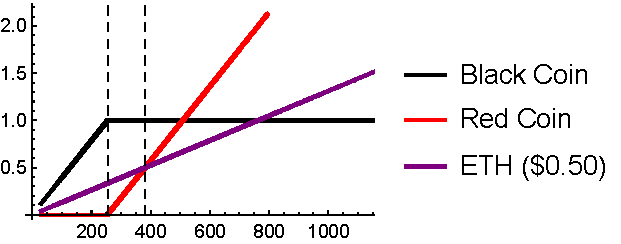
\includegraphics[height=2.5cm]{figures/price1.pdf}}
        \qquad
        \subfloat[A red coin, ETH equivalent to \$1.50, and a portfolio of a red coin and \$0.94.]{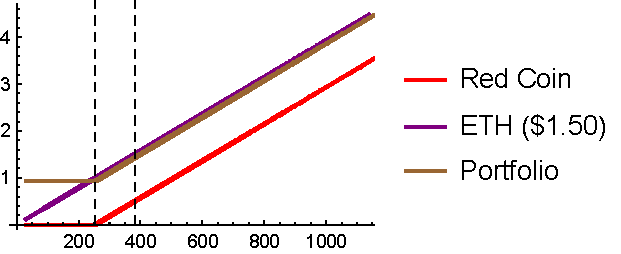
\includegraphics[height=2.5cm]{figures/price2.pdf}}
    \caption{Redemption value in USD (y-axis) as the price of ETH (x-axis) changes. \label{fig:price1} \label{fig:price2}}
\end{figure}

In this section, we answer questions about the financial characteristics of the red-black primitive. Consider a black coin that targets \$1 USD when 1 ETH is \$381.56 USD, and the DApp holds 0.00393126 ETH (worth \$1.5 USD).  Assume for now that (i) a red-black coin is a (non-fungible) contract between two individuals, and (ii) no one intervenes when ETH/USD declines enough that black coins starts to lose value (no liquidations). Figure~\ref{fig:price1}(a) shows how much a black coin is worth (y-axis) as the price of ETH varies (x-axis). The starting point (\$381.56 USD) is marked and if the price of ETH increases (rightward), the black coin is always worth \$1. If the value of ETH decreases (leftward), the black coin is still stable until the value of ETH hits \$254.37 (marked)---at this point, 0.00393126 ETH starts to become worth less than \$1 and the black coin `breaks the buck.'

Figure~\ref{fig:price1}(a) also shows the redemption value of a red coin. When created, a red coin is redeemable for \$0.50 USD. A user with \$0.50 USD can choose between purchasing a red coin or purchasing ETH (also shown). In both cases, the user profits when ETH increases and loses when ETH decreases in price. However the slope of red coin is greater. This indicates it is a \emph{leveraged} position in ETH.  

% = = = = = = = = = = = = = = = = = = = = = = = = = = = = = = = = = = = = = = = = = =

\subsection{How much should you pay for a black coin?}

Consider a black coin that is purchased today when ETH is \$381.56 USD. How much will it be worth in 100 days? In most future worlds, the black coin will be worth \$1. In some future worlds (when ETH is worth less than \$254.37), the black coin will break the buck. But even here, it takes a `haircut' on value as opposed to being worthless (\eg it can be redeemed for, say, \$0.90). 

\begin{figure}[t]
    \centering
        \subfloat[Price of ETH in USD (y-axis) over number of days (x-axis).]{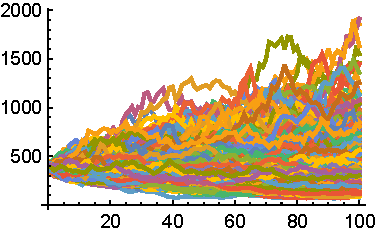
\includegraphics[width=0.4\columnwidth]{figures/mc.pdf}}
        \qquad
        \subfloat[Histogram of final price of ETH in USD (x-axis).]{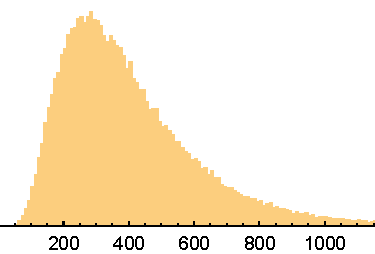
\includegraphics[width=0.4\columnwidth]{figures/histro.pdf}\label{fig:histro}}
    \caption{ETH/USD Monte Carlo simulation results. \label{fig:sim}}
\end{figure}

The expected value of a black coin can be estimated if we have a statistical model for ETH price movements. In finance, many statistical models have been proposed for many assets. Pricing ETH remains an open research problem. Until future research from the finance community advocates for the most appropriate model, we will sketch in some concrete numbers using Geometric Brownian Motion (GBM), which underlies the Black-Scholes model for pricing options~\cite{BS73} and has been used for ETH in other work~\cite{GPH+20}. We omit the details of the model itself (covered in nearly every  financial textbook~\cite{Sey09}). We fit the model to the historical `closing' prices of ETH for 1000 days prior to 18 Sept 2020\footnote{CoinGecko API: \url{https://api.coingecko.com}} and obtain $\mu=0.000744754$ (an upward drift in price over time) and $\sigma=0.0524172$ (a measure of volatility). If we simulate the next 100 days using Monte Carlo, we obtain the results in Figure~\ref{fig:sim}. For the parameters of this example, the expected value of the black coin is \$0.94 USD. Our model can be adjusted for the initial price, over-collateralization ratio (section ~\ref{sec:redchar}), and days until redemption. It is available in Python and Mathematica.\footnote{GitHub: URL omitted for anonymity.} 

As shown in Figure~\ref{fig:sim}\subref{fig:histro}, the expected return is log-normal. When we model more than 100 days, the variance increases and the expected redemption value of a black coin decreases: \$0.94 USD after 100 days, \$0.85 USD after 200 days, and \$0.80 after 1 year. This does not mean the black coin is worth less over time, it means the risk it falls out-of-the-money increases the more time you give it. 

% = = = = = = = = = = = = = = = = = = = = = = = = = = = = = = = = = = = = = = = = = =

\subsection{Why would you want a red coin?}
\label{sec:redchar}

While a stablecoin has utility to the holder, it is less clear what the utility of a red coin is. A red coin is a \textit{leveraged} position in ETH, which means that both gains and losses are amplified---compare the slope of the red coin value with a \$0.50 ETH investment at the same starting point (\$381.56 USD) in Figure~\ref{fig:price1}(a). Leverage is popular with investors. Investing in a red coin is equivalent to investing \$0.50 along with borrowing $2\times\$0.50$ in ETH (\ie 3:1 leverage). If the over-collateralization ratio is decreased from 1.50 to 1.10, then leverage for the red coin increases to 11:1. However, the black coin becomes riskier and its 100-day expected value drops from \$0.94 to \$0.86. For a \$2.00 collateralization, red coin leverage is 2:1, and the black coin value is \$0.98. 

Speculators seek out red coins but what about a user that wants to hold ETH without any leverage? She seemingly has no interest in red (or black) coins. Consider two scenarios: (a) she holds \$1.50 worth of ETH; and (b) she takes her \$1.50 worth of ETH, issues and sells a black coin (\eg for \$0.94 USD), and holds the red coin. She actually has a small portfolio of a red coin and close to \$1 USD. The redemption value of (a) and (b) are depicted in Figure~\ref{fig:price2}(b), along with the red coin by itself. The portfolio is actually an attractive investment---she has `insurance' against catastrophic loss during a devaluation of ETH for a small fixed `fee'---the \$0.06 USD difference between what she received for the black coin (\$0.94) and what the DApp pays out to the black coin holder (\$1.00). Additionally, she produced a stable black coin, which has external benefit to the decentralized economy. 

%With decentralized lending protocols (\eg Compound), red coins can earn interest with the same mechanism used for ETH, and the USD can also earn a return.

% = = = = = = = = = = = = = = = = = = = = = = = = = = = = = = = = = = = = = = = = = =

\section{Extending Red-Black Coins}
\label{sec:taxonomy}

Red-black coins are primitives. Other aspects of their design should to be considered before they actually are deployed. Design decisions include the maturity/redemption policy, how to make black and red coins fungible, and interventions to prevent the black coin from breaking the buck. One path through the decision tree leads to a design like Makers's \dai, however there are many other decisions that could result in very different stablecoins that have not been thoroughly explored by academics or the DeFi community to our knowledge.

%The purpose of this section is to emphasize that \dai is one set of reasonable decisions but there are many alternative designs that have not been (to our knowledge) explored.

% = = = = = = = = = = = = = = = = = = = = = = = = = = = = = = = = = = = = = = = = = =

\subsection{Fungibility of Black Coins}

Assume Alice creates a red/black coin, selling the red coin to Carol. Later, Bob creates a red/black coin, selling the red coin to David. Alice's black coin is not identical to Bob's black coin. Because they were created at different times, the ETH/USD exchange rate is different, and thus the  amount of collateral in ETH in the DApp will be different. The more collateral, the more a black coin is worth (recall Section~\ref{sec:redchar}). Such coins are not interchangeable or \textit{fungible} which adds effort to valuation and exchange. 

One design option is to \textbf{(1) forgo fungibility} and have each coin pair be its own individual contract between two counter-parties. This is the principle of forward contracts \cite{Har03}. A second option is to \textbf{(2) pool the collateral} of the red coins so that each black coin is a claim against the pool. A pool can be unfair: if Alice obtains a black coin before an ETH/USD price bubble, she is not exposed to the bubble bursting (assuming it returns to the pre-bubble price). However in a pool, all the black coins issued during the rising bubble are backed by significantly less collateral and when the bubble bursts, the pool becomes under-collateralized. The losses are democratized to all black coin holders including Alice. 

% = = = = = = = = = = = = = = = = = = = = = = = = = = = = = = = = = = = = = = = = = =

\subsection{Redemption}
\label{sec:maturity}

A policy for redeeming the collateralized ETH is the first design decision. Note that the DApp can autonomously distribute the collateral without the participation of the red or black coin holder, however someone needs to trigger a function call against the DApp to finalize the process.

 Red-black coins could \textbf{(1) mature on a pre-specified date} (\eg the first day of a specified month). At any given time, red/black coins in circulation would have one of a few different expiration dates, while still allowing some degree of fungibility. Coin holders would shorten or extend their coins by trading for a coin with a different maturity date. This is precisely how futures \cite{Har03} mature, and yTokens are based on the same principle~\cite{RoNi20}. After maturity, the DApp would lock all transfer functions and only allow withdrawal by the coin holders. The first to ask for a withdrawal would trigger the DApp to look up the ETH/USD price as of the maturity date and split the collateral accordingly. 

Alternatively, red-black coins could be redeemed at any time \textbf{(2) on demand by the black coin holder}, or \textbf{(3) red coin holder}, \textbf{(4) either}, or \textbf{(5) both}. Options (in the US style) \cite{Har03} work on the principal of (2) or (3), and price of a coin (\cf derivative~\cite{Sey09}) that is redeemable on-demand strengthens. Allowing either to redeem is unlike anything we could find in traditional finance---we speculate it would add uncertainty without any clear gain. Requiring both to agree to redemption is not actually an agreement \textit{per se}, the idea is a black coin holder would purchase a fungible red coin (or conversely, a fungible black coin for a red coin holder) and redeem the collateral on-demand. This is how \dai works, using fungible black coins and non-fungible red coins. 

% = = = = = = = = = = = = = = = = = = = = = = = = = = = = = = = = = = = = = = = = = = = = = = = = = =


\subsection{Under-collateralization}

When the ETH/USD exchange rate drops enough that under-collateralization is possible, the system could \textbf{(1) do nothing} and let the black coin holder price the risk of this into the coin, or the design could attempt further mitigation. In traditional financial markets, exchanges attempt to quickly liquidate a trader's losing position when the trading account balance dips below a threshold. Similarly, the DApp could require red coin holders to top-up their collateral and \textbf{(2) liquidate} it (\eg sell it by auction for black coins) if they do not. When collateral is pooled, this is crucial because under-collateralized red coins hurt all black coin holders. When collateral is not pooled, liquidation is useless for black coin holders because both ETH and black coins decrease in value at the same rate (recall Figure~\ref{fig:price1}) so it is simpler to do nothing.

Liquidation does not incentivize topped-up collateral unless it is accompanied by a \textbf{(3) punishment} (otherwise red coin holders might try to buy their liquidated assets from themselves at a discount). Beyond charging a fee, a stablecoin system might also withhold rewards (some systems used a secondary token for providing governance and providing rewards) or block red coin transfers until collateral is restored. In traditional financial markets, it is also the case that a trader's margin is inadequate to settle their account, they are still legally liable for the difference. A stablecoin accompanied by a \textbf{(4) reputation system} could mandate that red coin holders settle any obligation, however this increases the bound on how much a red coin holder can lose. A different approach is to obtain \textbf{(5) insurance} or financial coverage for the event of a decline in ETH/USD. This could be actual insurance, whether decentralized or through a traditional brokerage, or an offsetting financial investment that hedges the currency exchange risk.

The last approach is \textbf{(6) bail out} any losses through sales of a secondary token. This was used recently by Maker for \dai holders when its normal procedures of (2) and (3) were not adequate for dealing with a sharp, unexpected decline in the price of ETH on 12 Mar 2020 (`black Thursday'). While the auction was successful and recollateralized the pool, it cannot be generally guaranteed that minting new tokens will always be adequate for offsetting any debt. This event also exposed the lack of understanding and underestimation of risk by many vault (\ie red coin) holders who faced losses under (3), and raises the question of whether a system should be designed that is more forgiving to red coin holders in turbulent markets, especially since their financial position enables the issuance of a stablecoin. 

% = = = = = = = = = = = = = = = = = = = = = = = = = = = = = = = = = = = = = = = = = = = = = = = = = =

\subsection{Autonomy} 

The red-black coin primitive is entirely autonomous, which can be instantiated in a DApp and operate without human intervention. While the core primitive provides price stability, traders who are time-sensitive may forgo obtaining a good price in order to trade quickly. This particularly is influential for stablecoins which provide a low-friction avenue in and out of speculative positions on the price of ETH. Since red and black coins are issued in the same proportion, supply/demand imbalances between them add volatility to the black coin price. This could potentially be addressed in the design. 

A non-interventionist approach would let the red and black coin price \textbf{(1) float freely}. This avoids adding complexity to the design, and a design goal might be a system traders can easily understand and grasp the risk of. An alternative is to further stabilize prices by \textbf{(2) setting rates and fees} at various points in the system. For example, if black coin holders can redeem at any time, a fee could be charged to the black coin holder and paid to the red coin holder. If redemption requires both a red and black coin, the fee could be collected by the DApp. This principle is used by central banks for targeting interest rates, and is used in Maker to control the spot market for \dai. It is a struggle to set fees in the context of a decentralized and autonomous organization---while allowing decisions to be voted on is a first step, it does not guarantee that token holders are independent, informed, and not unduly influenced by the `expert' recommendations. 

% = = = = = = = = = = = = = = = = = = = = = = = = = = = = = = = = = = = = = = = = = = = = = = = = = =
% = = = = = = = = = = = = = = = = = = = = = = = = = = = = = = = = = = = = = = = = = = = = = = = = = =
% = = = = = = = = = = = = = = = = = = = = = = = = = = = = = = = = = = = = = = = = = = = = = = = = = =

\section{Concluding Remarks}

In this paper, we distil complex stablecoin systems into one of their core primitives, the red-black coin and provide a detailed study of its characteristics and possible extensions. It would be useful to have research results on the most suitable financial model for the ETH/USD price rate (\eg drift-diffusion models instead of simple GBM) for us to use in work like this paper. Future work could also examine the benefits of building a \dai alternative, still based on red-black coins but using different design parameters. Two examples that seem interesting are: (a) a more understandable system that reduces the amount of intervention, and (b) a system with fungible red coins that can be traded freely. Finally, while our paper answers the question of how much you should pay for a black coin, the analysis is much more complicated for \dai---with pooled collateral, liquidation, and bailouts, \dai is less risky than a simple black coin but the risk that these countermeasures systemically fail is not zero.


%



\section{What is RB tokens}
%%"A currency, to be perfect, should be absolutely invariable in value," said David Ricardo in 1817.
%%There is a huge debate about the charectaristics of a stable asset. One may claim that a stable asset or currency is an asset that helps its owner to have stable purchasing power. Others may claim that an stable asset should have invariable quantity.

There is a growing tendency to issue asset on top of blockchain that represents  real world assets such as shares, commodities, and currencies. 

One way to implement this kind of tokens is that a company obtains a reserve of the asset and issue tokens that represents a unit of asset. But this design needs custodianship proofs, periodic audits and also trust on the third party.

The question raised here is whether it is possible to find a solution to remove the trust on the third party?

The answer is RB token Dapp. There are two parties involving on each contract of the system. The Red token holder who need a representation of the underlying asset on the blockchain, and Black token holder who bets against the pair value of ETH and the underlying asset.

Therefore, the amount of deposited ETH on each new agreement will grow or shrink depending on the exchange rates of the underlying asset and ETH. Because a blockchain has no inherent knowledge of exchange rates, this mechanism still requires one trustworthy entity called an oracle to write the exchange rates into the blockchain (or consensus can be taken across a set of oracles).

\emph{Working Example}: Assume Alice wants to create representation of Google share (GOOGL). She sets up a DApp that can hold ETH and issue tokens. The DApp determines how much ETH is equivalent to 1.5 GOGGL, using the current exchange rates, provided to the DApp by a trusted third-party oracle, and Alice deposits this amount of ETH into the DApp. The DApp issues to Alice two tokens, Red and Black. At some future time, the holder of Red token can redeem up to equivalent value of 1 GOOGL in ETH from the deposit and the holder of the Black token gets any remaining ETH. Alice will transfer the Black token to Bob who wants to bet against ETH/GOOGL. When Alice redeems the Red token, it will be worth 1 GOOGL in ETH when the entire deposit of ETH is worth more than 1 GOOGL. If the exchange rate of ETH drops enough or the exchange rate of the GOOGL raise enough (or combinatoion of them), the entire deposit will be worth less than a 1 GOOGL—Alice will get all of the deposit, and the holder of the Black token will get nothing.

There are two risks on the system: Volatility risk of ETH and the underlying asset. Decision on the system depends on the spot exchange rate of ETH and Underlying asset
($\frac{P_{ETH}}{P_{GOOGL}} $).


\section{Analysis}



\section{Systemization}
There are a number of stablecoins using crypto-assets as collateral to issue stablecoins which shows a very broad design landscape for indirectly-backed stable coins and different design goals and strategies behind stable coin systems. In this part we will discuss about the mechanism that could be added on top of the RBcoin system discussed on previous section that can be used to change the propetries of the system. The designer of a stable coin may have design goals like Fungibility(I think it should be removed)(Money like tokens could be replaced or sth like that), Stability, Simplicity, and Decentrality. 

Firstly, the designer sets the goals of the design and then assign the design parameters of the system to acheive the design goals.

In this part, we propose a systematical design-decision model for indirectly-backed stablecoins. The designer is facing four main design parameters to create a new indictly-backed stable coins which are Maturity date, Counter-party, Collateral risk and interventions. 



An overview of the indirectly-backed stablecoins design landscape is in Figure\ref{land}.

\begin{figure} 
\centering
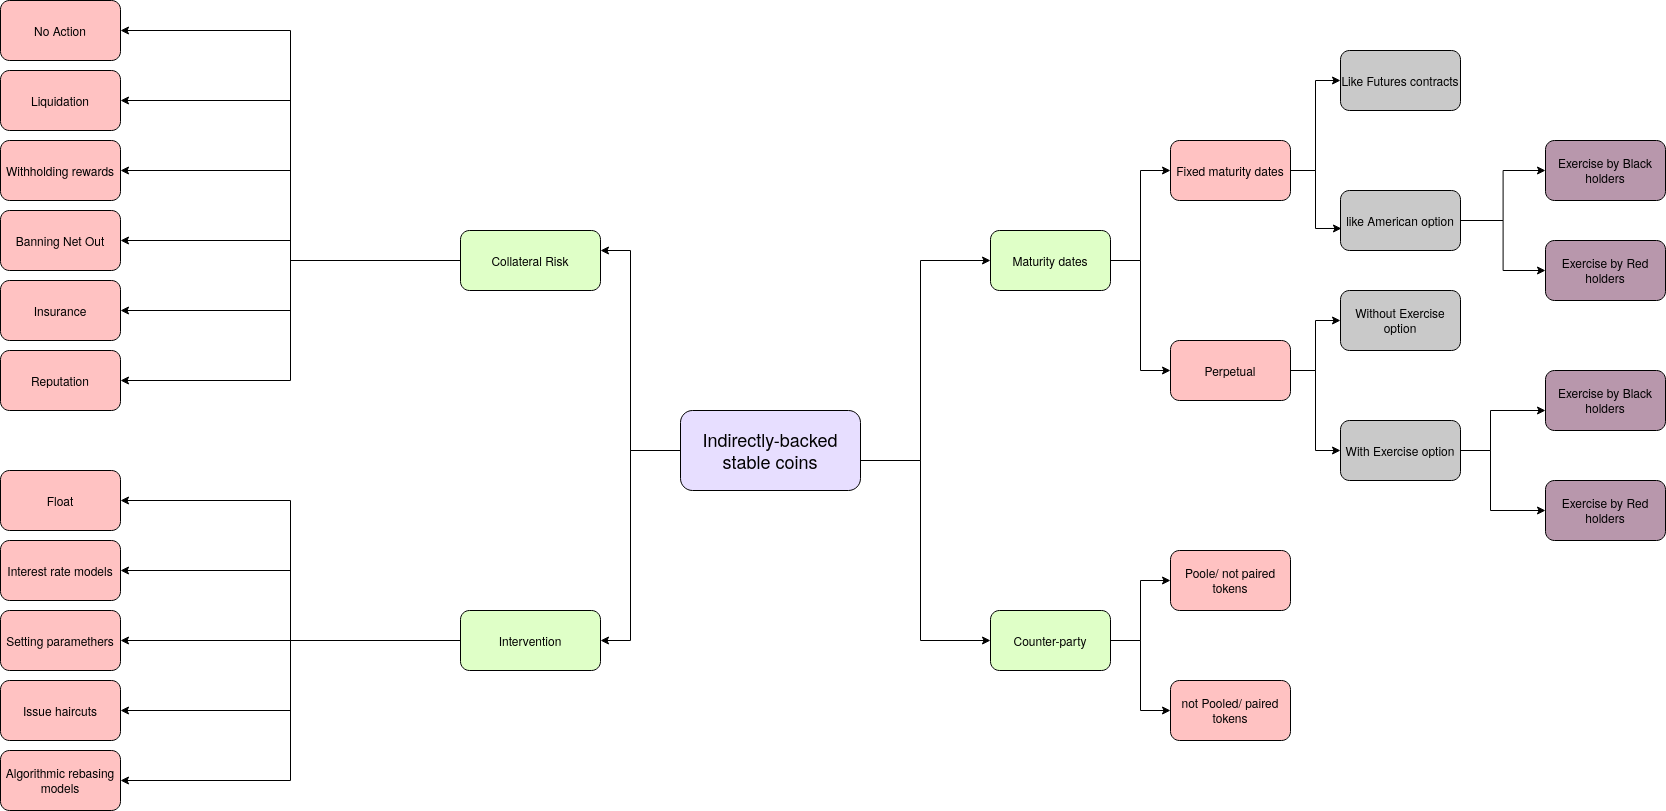
\includegraphics[width=12cm]{Mindmap}
\caption{overview of the indirectly-backed stablecoins design landscape}
\label{land}
\end{figure}

\subsection{Maturity Date}
The indirectly backed stable systems are agreements between two different parties, a stable party and a volatile party. These two parties should be different because holding both sides of the contract is equal to keeping the underlying asset on the wallet and it is not logical to participate on such a system to just keep the asset.

In this agreement the parties agree to split their deposited asset at a specified date named maturity date. At the maturity date the stable party will receive an exact amount of underlying asset based on the price of the asset at the settlement date and the volitile party will receive the remained part.

The first parameter that the designer should decide about is the maturity date. The maturity could be happened at a fixed specific time or could be perpetual.
\subsubsection{Fixed Maturity dates}
The designer can set specific dates for the contracts to be matured for example at the first day of each months. At the day of maturity the deposited assets are devided into two parts. The \$1 equivalent amount of the asset goes to the pocket of the stable party (if possible) and the remained is for volatile party. This is simlar to futures contract in Finance.

The designer may let one of the parties to exercise the contract beforr the maturity date. It is very similar to american options. The exerciser could be the black coin holder, red coin holder or both of them. 

\subsubsection{Perpetual contracts}
The other way to design the stable coin contracts is to make them as a perpetuty. In this mechanism there is no specific day for the parties to mature the contract. The system may have the option of settlement.

The perpetual stable coin without settlement is not rational because it is like burning the underlying asset to issue stable coins. 

For open-ended perpetual stable coins one of the parties has right to request for settlement whenever she wants. The exerciser could be black coin holder or red coin holder.
\subsection{Counter party}
One of the design parameters is to decide who is the risk taker in each contract. Each newly issued contract is backed by a different vault. Each black coin points its vault because the amount of deposits depend on the black coin holder decision. 
The designer could decide whether use a pool for red coins or pair each red coin to its related black coin.

\subsubsection{Pooled}

In this type of design the black coins are pointing to the vaults. Red coins are fungible on the system and there is no differences between them. There is no relations between red coin and the black coin. 

In this class, all red coin holders are risk takers of the system and on the unexpected events the take the risks regardless of their issuance contract.

In this case a black coin holder do not know the counterparty and the risk is pooled here.

\subsubsection{Paired}

The designer can create a system in which each red coin and black coins are paired and point to the issued contract. Now the black coin holders now their counterparty and the red coin holder is the risk taker of its own vault. So the risk is not pooled here.
\subsection{Collateral Risk}
If the price of the underlying asset goes down, the value of deposit falls below collateral ratio. The designers have the choice to react to this situation. We described some of different possible decisions:

\paragraph{Liquidation}
This variety of design is similar to the marginal accounts in traditional finance. If the underlying asset decreases in price and the value of a vault runs under the collateralization ratio, the system will liquidate the vault.

Liquidation occurs in the case that a vault is the danger area and may not able to pay its obligation. The deposited assets will transfer to the person who takes the responsibility of the debt of the vault. In other words, the liquidator should pay the borrowed red coin (and other obligations in a type of design, such as stability fee in MakerDAO) and receive the vault in exchange.


In liquidation design, the majority of vaults are over-collateralized. If a vault goes under-collateralize it will be liquidated. So, the red coin holders are pretty sure that their coin is backed by a dollar (. They can exchange their asset because the red coins are similar.

Smart contracts cannot trigger themselves. So, there should be an outsider player (like Keepers in MakerDao) to liquidate the warned vaults. They should trace the system to find the under-collateralized vaults and call the liquidation function. Then the keeper will transfer the debt of the vault to the smart contract and receive the deposit of the vault in exchange.

There are design parameters in the liquidation method:

\begin{enumerate}
  \item Collateralization Ratio:
This number shows the factor of over-collateralization. The ratio between the value of the deposits on each vault and the value of borrowed red coins should always be more than the collateralization ratio.
  
The collateralization ratio is depending on the volatility of the underlying asset. For instance, in the MakerDAO platform, the collateralization ratio for ETH vaults is 1.5. However, in the Synthetix project, it is 7.5 for SNX token, which is more volatile than ETH.
  \item Liquidation Incentive:
A smart contract is not able to trigger itself. An outsider player named liquidator should pay the transaction fee to call the liquidation function of the smart contract. Some factors influence the costs and profit of liquidators:
\begin{enumerate}
	\item Transaction fee:
The liquidator should trigger the liquidation function, send the sufficient red coins, and bid on the auction to win the vault. The user has to pay the transaction fee for these processes. The transaction fee depends on the time of transaction and network congestion.  
	\item Cost of capital: The liquidator pays the obligation by Red coin and receives the deposited coins of the vault. Therefore, the liquidator needs a sufficient amount of red coins for liquidation. There is an opportunity cost associated with the decision of the liquidator to not lend her capital and gain interest.

In other scenarios, the liquidator may just borrow the fund from lending platforms to liquidate the vault and pay back the loan afterward. There is a cost of borrowing in this scenario as well. So, there is a cost of capital for the liquidator.
	\item Price Oracles: RB coin systems need the price of the underlying asset in USD. Blockchains have no access to externals data. Oracles are outsider systems that collect the price and push them to the blockchains. Price inefficiency may impose extra costs on the liquidator. For instance, if the price of the asset is \$100 on the markets, although the oracle price is \$90, the liquidator spends more to provide liquidity from the markets.
\end{enumerate}  

The designer has to incentivize the liquidators to trace the blockchain, find alerted positions, and then send transactions to liquidate them. 

The mechanism of the incentivization is varied between protocols. A majority of platforms give the liquidator discounts on the vaults. For instance, in Single Collateral DAI (SAI), there was a \%3 discount on the liquidation process. Other platforms are using auction models to let the market decide about the value of the vault. 
  
  \item Auction model:
In the case of liquidations,  liquidators may come up with a specific warned position and want to liquidate it. The system designer has different options for the decision of picking the winner liquidator.
 
The simplest implementation mechanism is the First Come First Serve. However, it won't be fair for the vault holder if the first liquidator bids with a low amount of red coins.

There are other auction-based mechanisms to find the liquidator. The question raised here is, which method is the most efficient and fair auction model for both bidders and vault holders.

MakerDao utilizes a mixture of an absolute-auction and a reverse-auction model for the liquidation process.

The absolute auction model is used until the bids cover the debt of the vault. When the bids pass the debt, the auction reversed, the bidders bid on a lower amount of the deposits on the vault for a specific amount of DAI tokens, specified on the absolute auction step.
  
  \item Liquidation penalty:
The liquidation penalty is an extra punishment for the black coin holders to care about their debt to collateral ratio.
MakerDAO platform charges liquidated vault extra \%13 as a punishment for their vault holders. There are two main reasons to add Liquidation penalty on the design:

\begin{enumerate}

  \item To force vault keepers to be over-collateralized
  \item To mitigate grinding attacks: grinding attack occurs when the position holder deliberately unsafe her black coin and participate in the liquidation auction against her position to buy her deposited assets cheaper.

\end{enumerate}
\end{enumerate}

Using liquidation mechanism as a shield to protect the system provoke criticism. Possibly the black coin holders are freaking out when the price of ETH drops significantly. They may proceed to net out just before the liquidation occurs to their vaults. We called this situation "early liquidation" of the system. 

In this case, the system needs more ETHs to be deposited. The liquidation mechanism is designed to force the black coin holders to inject more ETHs to the system, but the black coin holders withdraw their deposits, and the total collateral of the system drops significantly, which is not the goal of the designers in this situation.

\paragraph{Withholding rewards}

Majority types of designs like liquidation are disincentivizing bad actors. But, another approach is to encourage users to act properly and incentivizing good actors of the system.

For instance, in the Synthetix project users need collateralize SNX tokens (Synthetix network token) to receive sUSD tokens (Synthetix stable coin pegging a USD). There is no margin call methods or liquidation function on the design. But, there is a reward on the system for users who keep more than the over-collateralization ratio. 
The Synthetix system has \%2 annual inflation on SNX tokens. The inflationary tokens are allocated to the vaults that hold more than the collateralization ratio.

There is another reward for the system. The traders on the exchange of the Synthetix project, pay transfer fees collected and distributed to the vaults holding more than the collateral ratio.

The system incentivizes people to stake their SNX token to be over-collateralized and receive the rewards. So, there is no punishment in the system for bad actors in this class of design.

\paragraph{Banning Black coin holders}

In the design of indirectly-backed stable coins, the red coins are not redeemable. In other words, the red coin holders cannot give back their red coins to receive \$1 of the deposited ETH in exchange. The red coin holder must own (or buy if possible) a black coin to net out a vault and receive the ETH.

In the liquidation scenario, the designer pushes black coin holders to be over-collateralized, applying liquidation punishments. Red coin holders and arbitragers are confident that there is no difference between the red coins because each of the red coins is backed by a sufficient amount of ETHs to be \$1 (with high probability).

In another class, the designer removes the liquidation mechanism, prevent black coin holders from withdrawal. In the fungible black coin design class, the designer also forbids the black coin holders from transferring their token. 

In this situation, the incentives for black coin holders to be over-collateralized has been decreased, compared to liquidation design class. But, there is a huge incentive left for them to be over-collateralized. If the price of the underlying asset drops, the black coin holders may want to sell their deposited assets to reduce the loss. In this scenario, just black coin holders that have over-collateralized vaults can net out and receive their underlying assets to sell them to the market.

This type of design will increase the fluctuation of the price of the red coin. The market watches the aggregated collaterals on the system and the number of red coins issued by the system and also the price of the underlying asset to evaluate the price of red coins. So when the price of underlying asset drops, the price of red coins will reduce concerning the underlying asset price. 

In this scenario, red coin holders are taking parts of the risk of underlying asset volatility risk. On the situation that the price of the asset drops significantly, the value of the stable coin will fall.

\paragraph{Reputation systems}

In traditional finance, reputation scoring systems are used to decrease or eliminate the collateral needs for a specific financial transaction. Participants are utilizing their reputation as collateral or source of trust for financial services. 

For instance, in the FICO credit score system, users can enhance their credit limit by increasing their credit score. There is a default risk on credit systems, but the defaulted person will be punished by credit score reduction. The bad actor loses reputation scores forbidden from using plenty of financial services. Therefore, users have adequate incentives to pay their bills.

A revolution of decentralizing the finance products on top of blockchain technologies began in early 2018, named Decentralized Finance (Defi) movement. There is a myriad of different decentralized financial services out there, such as MakerDAO, Compound, Synthetix, Aave, etc. 

There are no differences between users that act properly on Defi platforms and the bad actors. The DeFi ecosystem suffers from a lack of a reputation system or reputation scoring. Using a reputation system will incentivize users to act properly and also reduce the default risk of the system. On the other side of the coin, the users with high-grade reputation scores have new opportunities. So, the cost of defaulting will be increased for high-grade users.

There are barriers to implementing an effective reputation system on blockchains. Lack of strong identities or anonymity is one of them. Also, users can create fake histories. However, these are not impossible to address.

In case that our system concludes a trustworthy reputation system, the designer can use reputation as collateral.  We describe two different designs using reputation systems:
\begin{enumerate}
	\item Reputation-based collateral ratio: 
In the design of the system, the collateral ratio could be reliant on the reputation of the user. In other words, the collateral ratio is higher for new users (users with no reputation) and lower for users that act properly for a long time.
	\item Reputation-based staibility fee
In systems like MakerDAO, the DAI borrowers are obliged to pay a fee on their borrowing named stability fee. This stability fee is being set by Maker token holders.
	In a design based on the reputation, the stability fee could be dependent on the reputation of the user. The reputable user is paying a lower stability fee compared to the new users.
\end{enumerate}
 
\paragraph{Insurance}
Insurance models are used to hedge the risk of unexpected events in different systems. Under-collateralization of a vault is an unexpected event on the RBcoin system. The designer could use an insurance model to protect parties from financial loss in the case of under-collateralization. 

On the insurance model, the insurer will pay a premium to the insurance company. The company will protect the client from financial loss. 

In RBcoins there could be a built-in or outsourced insurance model to protect parties from under collateralization loss. The question raised here is who should pay the premium.

\begin{enumerate}
	\item Premium pay by Red coin holders:
It is very similar to Credit Default Swaps (CDS) on traditional finance. In this design, the approach is that the red coin holders are lending some amount of money to black coin holders. Therefore, black coin holders are borrowing from red coin holders to have a leveraged position on the underlying asset. In this situation, the red coin holders can pay an insurance premium to the contract to protect themselves from the default risk of black coin holders. In the case of under-collateralization, if the black coin holder cannot afford the loss, the insurance contract will pay the loss to the red coin holder.

This type of design is implemented on the MakerDAO platform. The DAI borrowers are paying a premium so-called stability fee to the system. These fees are collected on a pool named Maker Buffer pool. In the case of liquidation of a CDP, if the winner of the auction pays a lower amount of the obligation of the vault, the difference between the obligation and the paid amount will be paid by the Maker Buffer pool.

	\item Premium pay by Black coin holders
In this type of design, the black coin holders are paying the insurance premium. It is similar to regular insurance contracts in which the insurer buys an asset and guarantee it by paying a premium to insurance companies. For example, a person purchases a house and insure it.
Here the black coin holders are buying a position and pay the insurance premium. If the price of underlying asset drops and the vault going to be liquidated the insurance contract will pay on behalf of the insurer.
	\item Premium pay by both
In this scenario, both Red and Black coin holders are paying the insurance premium to ensure their positions. 
\end{enumerate}
\subsection{Intervention}

The designer should indicate the level of intervention on the system. There could be some mechanisms to change the level of properties on the system. For instance, the designer may use interest rate models, algorithmic models or secondary tokens to acheive a system property.

\subsubsection{Float}

The desiner may let the system to be free of human or algorithm intervenions. This is the most decentral type of design. This type of design benefits simlicity and decentrality but the red coins has fluctuations.

\subsubsection{Interest rate models}

Interest rates are tools that a system governer has to stimulate the demand or supply side of a system. The designer of indirectly-backed stable coins can use interest rate models on red coins or black coins (two different rates) to adjust the supply and demand of black coins and red coins in the system. This rates could be adjusted by human intervention like DAI or could be fully algorithmic.

\subsubsection{Parameter setting}

All types of the indirectly-backed stable coin system has some parameters in common such as collateral ratio. In specific designs, there are other design parameters added to the system such as maturity dates, insurance premium and rates. The designer may decide to intervene on the system and change these parameter over time. This intervention could be by humans or algorithmic. 

\subsubsection{Issue haircut}

The designer should indicate that in case that the price of underlying asset goes down, who is the risk taker of the system. On regular system risk taker of the system is black coin holders till the price falls strongly and the black coins worth zero, then the red coin holders take all the risk.

The designer has other option to divide the risk between red coin holders and black coin holders. The designer could set hair cut parameter a (< 1). It means that if the price of the underlying asset falls 1 percent the redcoin holder now takes a percent of the risk and the the black coin holder takes 1-a percent.

This haircut parameter could be changed during the time by human intervention or algorithmic.


\subsubsection{Algorithmic rebasing models}

The designer may use rebasing models to change the number of tokens in a way that at the end of each day the price of redcoins is exactly a dollar.

%\section{Design Landscape}
The purpose of designing a crypto-asset backed stablecoin is to create a stable asset out of a volatile asset. There are a number of stablecoins using crypto-assets as collateral to issue stablecoins which shows a very broad design landscape for indirectly-backed stable coins.

In this part, we propose a systematical design-decision model for indirectly-backed stablecoins. There are some key design decisions for each core feature. We describe core features and the key design decisions related to the main features, and also we will discuss the pros and cons of each feature.

An overview of the indirectly-backed stablecoins design landscape is in Figure \ref{land}.

\begin{figure*} [ht]
\centering
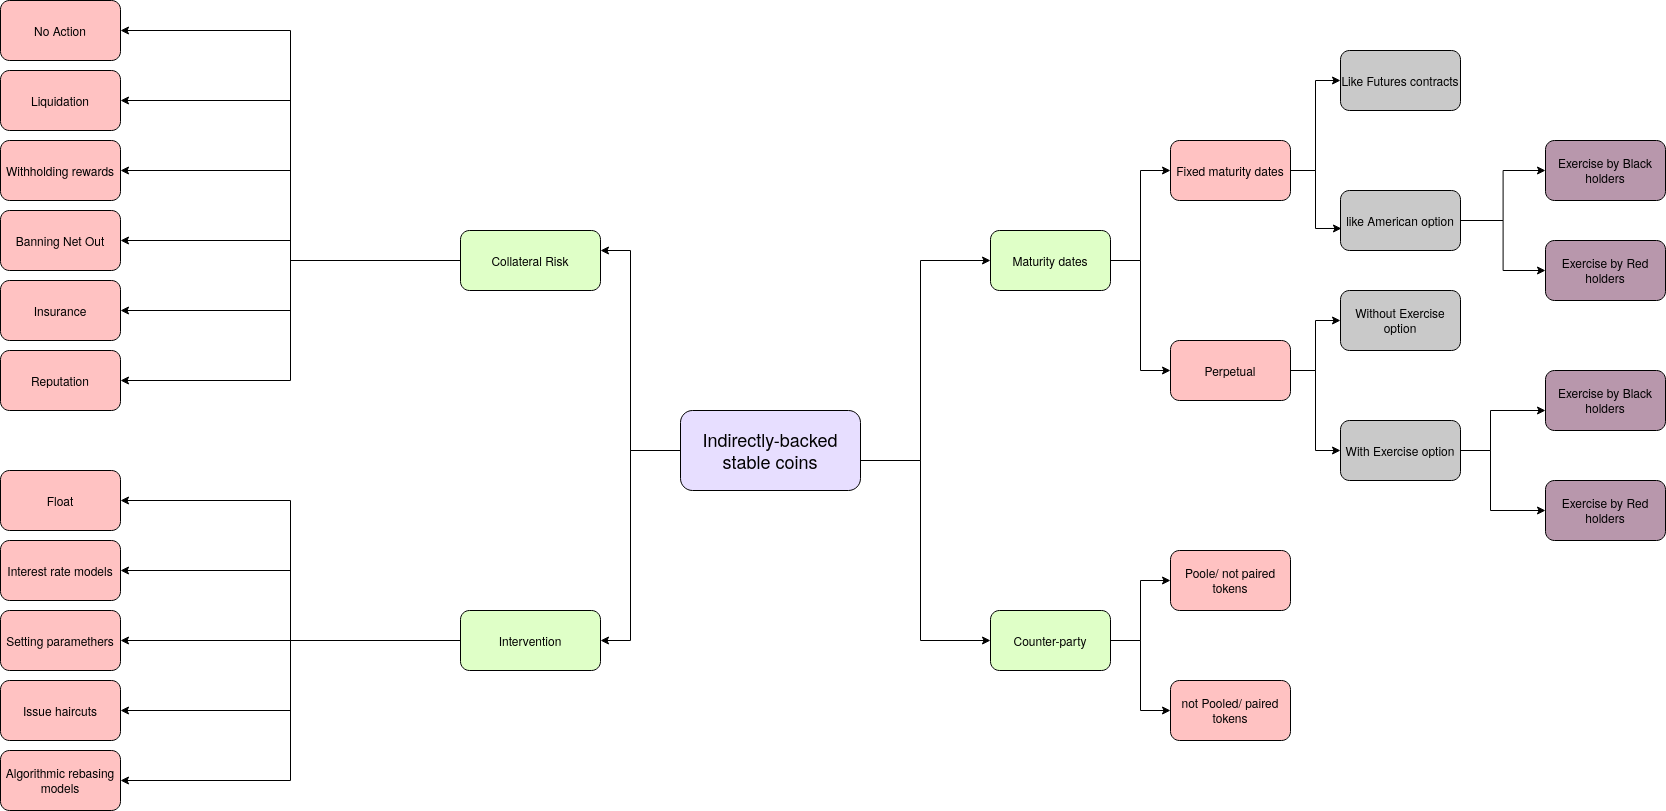
\includegraphics[width=16cm]{Mindmap}
\caption{overview of the indirectly-backed stablecoins design landscape}
\label{land}
\end{figure*}

\section{Fungibility}
Fungibility or Interchangeability refers to the feature of an asset to be exchanged by the same asset type with equal quality and quantity. For instance, dollar bills are fungible because people can exchange the same amount of dollars without any frictions.

The first design decision is whether the tokens on the systems should be fungible or should be non-fungible. 

Fungiblity decision is devided into two parts:
\begin{itemize}
  \item Red coins Fungibility
  \item Black coins Fungibility
\end{itemize} 
We will discuss them seperately on next sections.


\subsection{Red coins Fungibility}
The Red coins, the stable coin of the system, could be fungible or non-fungible. All currently implemented indirectly-backed stablecoins are using fungible stablecoin design. However, it could be non-fungible as well.

\subsubsection{Non-fungible Red coins}
A stablecoin system designer could allow red coins to be non-fungible. For instance, each token could be backed by a different amount of ETHs without limitations on the system such as collateral ratio, liquidation and etc.

In this design class, the Red coin and Black coin should be pair-wise. Because each pair is backing by a different vault and a specific amount of deposited ETH.

There should be a system parameter for each red coin, depends on its vault to distinct the coins.
For example, each red coin could be marked by debt to collateral ratio, the number of minted red coins divided by the value of deposited ETH on the related vault, which clarifies the safeties of the coin.
So the buyer could have speculation on the price of each red coin base on the debt to collateral ratio.

Some reasons push designers to make red coins fungible. The first reason is usability. Assume that Alice wants to buy 100 red coins. On the other side, Bob wants to sell just 30 coins, Carol wants to sell 50 and David wants to sell 20 red coins. Now Alice should make a price speculation of three different coins and buy them at different prices which is not convenient for her.

The other issue with the non-fungible red coins is price discovery. Markets and crowd wisdom help to aggregate different opinions on the value of an asset. The aggregated results will discover the efficient price of the asset. In non-fungible design, there is not a straight relation between the price of each red coin and the specific characteristic of them like the debt to collateral ratio. So, Each person has speculation for each coin. Because of non-fungibility, the aggregations would not happen and so the real price will not be discovered.

The other reason is that stable coin users are willing to use the stable coins as a money. So, they need stable coins serve as a unit of account which means that you can price other goods or assets using the stable coin. In non-fungible design each red coin has a specific price. So, users can not price other goods based on the stable coin.


\subsection{Fungible Red coins}
As mentioned in the previous part, stable coin designers put all their effort to create stable coin systems including fungible red coins. There are different mechanisms to bring fungibility into red coins. We classify them into two key designs discussed in the next sections.

\begin{itemize}
  \item Under-collaterallization
  \item Separate maturity dates
\end{itemize} 


\subsubsection{Collateral Value Assurance}

One of the methods to bring fungibility into red coins is to set a lower limit for vaults (Collateralization ratio). If the value of deposited ETH in a vault drops beneath a specific amount, then the system decides to take an action. 

In this circumstance, there is a minimum amount of ETHs (collateral ratio)  backing each red coin. It secures the fungibility of red coins. Red coin holders are sure that there is at least a dollar in the vault for their red coin  (strongly expected). There is no difference between their red coin and the red coin of other people in this circumstance.

We will discuss various designs that differ on how they secure the vaults from the under-collateralization in the next sections. Some of them are incentivizing vault keepers to keep their deposit more than collateralization ratio and some of them are disincentivizing the bad actors of the system.
 
\paragraph{Liquidation}
This variety of design is similar to the marginal accounts in traditional finance. If the underlying asset decreases in price and the value of a vault runs under the collateralization ratio, the system will liquidate the vault.

Liquidation occurs in the case that a vault is the danger area and may not able to pay its obligation. The deposited assets will transfer to the person who takes the responsibility of the debt of the vault. In other words, the liquidator should pay the borrowed red coin (and other obligations in a type of design, such as stability fee in MakerDAO) and receive the vault in exchange.


In liquidation design, the majority of vaults are over-collateralized. If a vault goes under-collateralize it will be liquidated. So, the red coin holders are pretty sure that their coin is backed by a dollar (. They can exchange their asset because the red coins are similar.

Smart contracts cannot trigger themselves. So, there should be an outsider player (like Keepers in MakerDao) to liquidate the warned vaults. They should trace the system to find the under-collateralized vaults and call the liquidation function. Then the keeper will transfer the debt of the vault to the smart contract and receive the deposit of the vault in exchange.

There are design parameters in the liquidation method:

\begin{enumerate}
  \item Collateralization Ratio:
This number shows the factor of over-collateralization. The ratio between the value of the deposits on each vault and the value of borrowed red coins should always be more than the collateralization ratio.
  
The collateralization ratio is depending on the volatility of the underlying asset. For instance, in the MakerDAO platform, the collateralization ratio for ETH vaults is 1.5. However, in the Synthetix project, it is 7.5 for SNX token, which is more volatile than ETH.
  \item Liquidation Incentive:
A smart contract is not able to trigger itself. An outsider player named liquidator should pay the transaction fee to call the liquidation function of the smart contract. Some factors influence the costs and profit of liquidators:
\begin{enumerate}
	\item Transaction fee:
The liquidator should trigger the liquidation function, send the sufficient red coins, and bid on the auction to win the vault. The user has to pay the transaction fee for these processes. The transaction fee depends on the time of transaction and network congestion.  
	\item Cost of capital: The liquidator pays the obligation by Red coin and receives the deposited coins of the vault. Therefore, the liquidator needs a sufficient amount of red coins for liquidation. There is an opportunity cost associated with the decision of the liquidator to not lend her capital and gain interest.

In other scenarios, the liquidator may just borrow the fund from lending platforms to liquidate the vault and pay back the loan afterward. There is a cost of borrowing in this scenario as well. So, there is a cost of capital for the liquidator.
	\item Price Oracles: RB coin systems need the price of the underlying asset in USD. Blockchains have no access to externals data. Oracles are outsider systems that collect the price and push them to the blockchains. Price inefficiency may impose extra costs on the liquidator. For instance, if the price of the asset is \$100 on the markets, although the oracle price is \$90, the liquidator spends more to provide liquidity from the markets.
\end{enumerate}  

The designer has to incentivize the liquidators to trace the blockchain, find alerted positions, and then send transactions to liquidate them. 

The mechanism of the incentivization is varied between protocols. A majority of platforms give the liquidator discounts on the vaults. For instance, in Single Collateral DAI (SAI), there was a \%3 discount on the liquidation process. Other platforms are using auction models to let the market decide about the value of the vault. 
  
  \item Auction model:
In the case of liquidations,  liquidators may come up with a specific warned position and want to liquidate it. The system designer has different options for the decision of picking the winner liquidator.
 
The simplest implementation mechanism is the First Come First Serve. However, it won't be fair for the vault holder if the first liquidator bids with a low amount of red coins.

There are other auction-based mechanisms to find the liquidator. The question raised here is, which method is the most efficient and fair auction model for both bidders and vault holders.

MakerDao utilizes a mixture of an absolute-auction and a reverse-auction model for the liquidation process.

The absolute auction model is used until the bids cover the debt of the vault. When the bids pass the debt, the auction reversed, the bidders bid on a lower amount of the deposits on the vault for a specific amount of DAI tokens, specified on the absolute auction step.
  
  \item Liquidation penalty:
The liquidation penalty is an extra punishment for the black coin holders to care about their debt to collateral ratio.
MakerDAO platform charges liquidated vault extra \%13 as a punishment for their vault holders. There are two main reasons to add Liquidation penalty on the design:

\begin{enumerate}

  \item To force vault keepers to be over-collateralized
  \item To mitigate grinding attacks: grinding attack occurs when the position holder deliberately unsafe her black coin and participate in the liquidation auction against her position to buy her deposited assets cheaper.

\end{enumerate}
\end{enumerate}

Using liquidation mechanism as a shield to protect the system provoke criticism. Possibly the black coin holders are freaking out when the price of ETH drops significantly. They may proceed to net out just before the liquidation occurs to their vaults. We called this situation "early liquidation" of the system. 

In this case, the system needs more ETHs to be deposited. The liquidation mechanism is designed to force the black coin holders to inject more ETHs to the system, but the black coin holders withdraw their deposits, and the total collateral of the system drops significantly, which is not the goal of the designers in this situation.

\paragraph{Withholding rewards}

Majority types of designs like liquidation are disincentivizing bad actors. But, another approach is to encourage users to act properly and incentivizing good actors of the system.

For instance, in the Synthetix project users need collateralize SNX tokens (Synthetix network token) to receive sUSD tokens (Synthetix stable coin pegging a USD). There is no margin call methods or liquidation function on the design. But, there is a reward on the system for users who keep more than the over-collateralization ratio. 
The Synthetix system has \%2 annual inflation on SNX tokens. The inflationary tokens are allocated to the vaults that hold more than the collateralization ratio.

There is another reward for the system. The traders on the exchange of the Synthetix project, pay transfer fees collected and distributed to the vaults holding more than the collateral ratio.

The system incentivizes people to stake their SNX token to be over-collateralized and receive the rewards. So, there is no punishment in the system for bad actors in this class of design.

\paragraph{Banning Black coin holders}

In the design of indirectly-backed stable coins, the red coins are not redeemable. In other words, the red coin holders cannot give back their red coins to receive \$1 of the deposited ETH in exchange. The red coin holder must own (or buy if possible) a black coin to net out a vault and receive the ETH.

In the liquidation scenario, the designer pushes black coin holders to be over-collateralized, applying liquidation punishments. Red coin holders and arbitragers are confident that there is no difference between the red coins because each of the red coins is backed by a sufficient amount of ETHs to be \$1 (with high probability).

In another class, the designer removes the liquidation mechanism, prevent black coin holders from withdrawal. In the fungible black coin design class, the designer also forbids the black coin holders from transferring their token. 

In this situation, the incentives for black coin holders to be over-collateralized has been decreased, compared to liquidation design class. But, there is a huge incentive left for them to be over-collateralized. If the price of the underlying asset drops, the black coin holders may want to sell their deposited assets to reduce the loss. In this scenario, just black coin holders that have over-collateralized vaults can net out and receive their underlying assets to sell them to the market.

This type of design will increase the fluctuation of the price of the red coin. The market watches the aggregated collaterals on the system and the number of red coins issued by the system and also the price of the underlying asset to evaluate the price of red coins. So when the price of underlying asset drops, the price of red coins will reduce concerning the underlying asset price. 

In this scenario, red coin holders are taking parts of the risk of underlying asset volatility risk. On the situation that the price of the asset drops significantly, the value of the stable coin will fall.

\paragraph{Reputation systems}

In traditional finance, reputation scoring systems are used to decrease or eliminate the collateral needs for a specific financial transaction. Participants are utilizing their reputation as collateral or source of trust for financial services. 

For instance, in the FICO credit score system, users can enhance their credit limit by increasing their credit score. There is a default risk on credit systems, but the defaulted person will be punished by credit score reduction. The bad actor loses reputation scores forbidden from using plenty of financial services. Therefore, users have adequate incentives to pay their bills.

A revolution of decentralizing the finance products on top of blockchain technologies began in early 2018, named Decentralized Finance (Defi) movement. There is a myriad of different decentralized financial services out there, such as MakerDAO, Compound, Synthetix, Aave, etc. 

There are no differences between users that act properly on Defi platforms and the bad actors. The DeFi ecosystem suffers from a lack of a reputation system or reputation scoring. Using a reputation system will incentivize users to act properly and also reduce the default risk of the system. On the other side of the coin, the users with high-grade reputation scores have new opportunities. So, the cost of defaulting will be increased for high-grade users.

There are barriers to implementing an effective reputation system on blockchains. Lack of strong identities or anonymity is one of them. Also, users can create fake histories. However, these are not impossible to address.

In case that our system concludes a trustworthy reputation system, the designer can use reputation as collateral.  We describe two different designs using reputation systems:
\begin{enumerate}
	\item Reputation-based collateral ratio: 
In the design of the system, the collateral ratio could be reliant on the reputation of the user. In other words, the collateral ratio is higher for new users (users with no reputation) and lower for users that act properly for a long time.
	\item Reputation-based staibility fee
In systems like MakerDAO, the DAI borrowers are obliged to pay a fee on their borrowing named stability fee. This stability fee is being set by Maker token holders.
	In a design based on the reputation, the stability fee could be dependent on the reputation of the user. The reputable user is paying a lower stability fee compared to the new users.
\end{enumerate}
 
\paragraph{Insurance}
Insurance models are used to hedge the risk of unexpected events in different systems. Under-collateralization of a vault is an unexpected event on the RBcoin system. The designer could use an insurance model to protect parties from financial loss in the case of under-collateralization. 

On the insurance model, the insurer will pay a premium to the insurance company. The company will protect the client from financial loss. 

In RBcoins there could be a built-in or outsourced insurance model to protect parties from under collateralization loss. The question raised here is who should pay the premium.

\begin{enumerate}
	\item Premium pay by Red coin holders:
It is very similar to Credit Default Swaps (CDS) on traditional finance. In this design, the approach is that the red coin holders are lending some amount of money to black coin holders. Therefore, black coin holders are borrowing from red coin holders to have a leveraged position on the underlying asset. In this situation, the red coin holders can pay an insurance premium to the contract to protect themselves from the default risk of black coin holders. In the case of under-collateralization, if the black coin holder cannot afford the loss, the insurance contract will pay the loss to the red coin holder.

This type of design is implemented on the MakerDAO platform. The DAI borrowers are paying a premium so-called stability fee to the system. These fees are collected on a pool named Maker Buffer pool. In the case of liquidation of a CDP, if the winner of the auction pays a lower amount of the obligation of the vault, the difference between the obligation and the paid amount will be paid by the Maker Buffer pool.

	\item Premium pay by Black coin holders
In this type of design, the black coin holders are paying the insurance premium. It is similar to regular insurance contracts in which the insurer buys an asset and guarantee it by paying a premium to insurance companies. For example, a person purchases a house and insure it.
Here the black coin holders are buying a position and pay the insurance premium. If the price of underlying asset drops and the vault going to be liquidated the insurance contract will pay on behalf of the insurer.
	\item Premium pay by both
In this scenario, both Red and Black coin holders are paying the insurance premium to ensure their positions. 
\end{enumerate}

\subsubsection{Separate Maturity Dates}
This kind of design employs the idea of Futures in traditional finance. Each contract is an agreement between a volatile and a stable party. They deposit an amount of ETHs on the system (Q). The strike price (K) is the dollar value of ETHs that the parties agree that the stable player will receive at the maturity date (M). The remained ETHs on the vault will go to the pocket of the volatile party.

For a specific amount of pooled ETHs, two tranches are created, the stable token and a volatile token (black token). Tranching in traditional finance is used when several securities are created from a pool of other assets, carrying different risks. The junior tranche (volatile token) takes the majority of the risk and the senior tranche (stable coin) takes a lesser risk.  

The stable tokens are not fungible because each represents a different maturity date.  To create a fungible stable coin, the stable tokens with different maturities are bundled to create the Red coin, stable coin of the system. The amount of red coins each user receives is depending on the maturity date and the strike price of the deposited stable coin.

For example, in the Lien project, the agreement between parties is that at the maturity day, the stable token holder will receive k USD if the deposited ETH worth k USD, and the surplus will belong to the volatile token holder. If the value of deposited ETH dropped below k USD then the stable token worth below K USD and the volatile token worth zero. There are different specified maturity dates every 2 weeks. When a party receives a stable token, she will deposit it on a smart contract named iDOL to receive the stable coin (iDOL token). The iDOL contract bundles stable tokens with different maturities and strike prices and issues a stable coin out of this basket.


\subsection{Black coins Fungibility}

The Black coins, volatile coin of the system, could be fungible or non-fungible. 

\subsubsection{Non-fungible Black coin}

In the majority of implemented indirectly-backed stable coin systems, such as DAI and sUSD black coins are non-fungible. The vaults in these projects are covering various amounts of ETHs. Consequently, the vaults are not fungible. 

Non-fungibility of black coins is one of the primary obstacles of the currently implemented projects. These systems are designed to attract users who need stability along with the features of cryptocurrencies. 

If Alice decides to issue new stable coins, first she requires to create a pair of a red coin and a black coin. She obliged to keep the black coin because black coins are not transferable. So, the users that need stability should wait till another person who is willing to open a leveraged position, create a new vault, and want to sell her red coins to the market.

The other problem of this kind of design is the control of the demand and supply of stable red coins. If the demand for red coins suddenly increases in markets, the price of red coins in markets will be increased. This is an opportunity for arbitragers to make a profit because the price of red coins is pegging a dollar. The arbitragers issue new red coins that cost \$1, sell the red coins to the market to make a profit. But, the problem raised here, because if the arbitrager creates a new vault, then she should hold a non-fungible black coin position. So, the arbitragers are not confident about the price of the red coins. Therefore, there is no motivation for them to make arbitrage on red coin markets.
 
The designers of the MakerDAO platform are using interest rate models to control the supply and demand for red coins and black coins. This core design feature will be explained in detail, in the next sections.

\subsubsection{Fungible Black coin}

Making black coins fungible is the way to solve the mentioned problem. If Alice wants a red coin, she can open a new vault, sell her black coin to the market, and then decide to use it or keep her red coin.

The fungibility of black coins could boost the market capitalization of indirectly-backed stable coins because people who are willing to use stable coins can issue new stable coins without friction.

In this sort of design, there is no need to adjust interest rates to control the demand and supply of red coins because if the price of recoins increases in a market, the arbitragers can create new vaults, sell the issued black coin to the markets and sell the newly generated red coin, which worths a dollar, to a person who is buying them more than a dollar. The arbitrager also could implement these steps in just one transaction, using the meta transaction method to save money on the transaction fees.

The problem with this type of design is when the demand for red coins increases, and there is no demand for black coins. So, the arbitrager should sell the newly generated black coin lower than the issued price.

However, it uses free-market decisions to calculate the price of red and black coins, which means if the price of red coin increases and there is no demand for black coins, the price of red coins will exceed a dollar. 

The other problem with this type of design is the transaction fee for arbitragers. Because the arbitragers are using meta transactions, they should pay high transaction fees for the arbitrage, which may not be profitable in such cases.
\subsection{Underlying asset}
The first decision that a designer should take is choosing the asset that the issuer use as collateral to issue new stable coins.

There is a strong dependency between the risk related to the underlying asset and the design parameters of an indirectly-backed stable coin.

The stable coins could be backed by a single asset, like SAI (the first version of DAI), sUSD, USDx. Or by a basket of different crypto assets like DAI. In multi-collateral backed stable coins, several design parameters depend on the assets used as collateral on the system. 

The purpose of using a basket of assets as collateral is to lower the risk impact of each asset on the stable coin. But the designers may forget the fact that there is a strong correlation between the price of assets. It means as the market of cryptocurrencies falls, all tokens drop in price. 

The underlying assets have two types:

\begin{itemize}
	\item \emph{Exogenous Asset}: Assets that have uses outside of the stable coin systems and just a portion of them are using as collateral on the stable coin system. For instance, ETH, BAT token, and KNC token are collateral options in the MakerDAO platform. These assets are designed to serve other projects, but users can use them as collateral to issue new DAI tokens.
	Another example is Binance token (BNB) used in the USDx protocol. 
	\item \emph{Endogenous Asset}: This class of assets is designed just to be used on the stable coin system. It means the majority of the assets are locked or used on the system. The Synthetix Network Token (SNX) is an example of endogenous assets. The SNX token is created to be used as collateral to issue new sUSD tokens, the stable token in the Synthetix project.
\end{itemize}



\subsection{Supply adjustment}
There is a class of stable coins named Money Supply Adjustment stable coins. In this type of design, the stability comes from the adjustment of the supply of the stable coin. In other words, in the case that the price of stable coin exceeds \$1, the system will increase the amount using a mechanism to reduce the price of the stable coin and vice versa. 

There is a difference between supply adjustment in indirectly-backed mechanism and Money Supply Adjustment method. In Money Supply Adjustment, there is just one coin (Stable coin) that the designer tries to adjust its supply. But, in Indirect-backed stable coins, there are two different tokens, red and black, that their quantity should be modified.

 In a bunch of indirectly-backed stable coins, the designer uses the supply adjustment mechanism to ensure the stable coin's price stability. For instance, in the MakerDAO project, there are two system parameters, Stability fee and Dai Saving Rate (DSR), to adjust the supply of the Dai stable coin.

There is a smart contract named DAI Saving contract or DSR contract. DAI token holders can lock their DAI tokens on the DSR contract and receive interest on the deposited DAI. It is very similar to Saving Accounts in banking. 
The stability fee is the fee that the Dai borrowers must pay back to the system. 

The MakerDAO system uses a combination of these two rates to adjust the DAI tokens and CDPs' supply. The stability fee is the tool to adjust the CDPs (black coins) and the amount of ETHs locked in the system. Decreasing the stability fee is an opportunity for users to create new CDPs with a lower cost of borrowing DAI tokens (red coins). If the Maker token holders conclude that the system needs new vaults, they can reduce the stability fee.
On the other hand, decreasing the DSR rate encourages the users that locked their DAI tokens on the DSR contract to withdraw their tokens and supply them to the market, which increases the supply of the DAI tokens.

The MKR token holders, governance token of the MakerDAO platform, can change. So the supply adjustment on the MakerDAO system is a human intervention mechanism. It has a conflict with the decentralization vision of the platform. Because the stability of the tokens is strongly dependant on the DSR and Stability fee, and humans are setting these two. However, the MakerDAO platform uses Decentralized Autonomous Organizations (DAO) to decentralize governance, but there is a critique, which we will discuss in the governance section.

The question here is, why do we need these two rates to adjust the supply of the DAI tokens. Assume that the demand for DAI tokens increases. The total supply of DAI should be increased, or the DAI price will exceed one dollar due to the supply and demand rule. So, arbitragers have an opportunity to make a profit. They can issue new tokens worth one dollar and sell them on the market, which increases the supply and reduce the price of the DAI token. However, there is a problem with arbitragers. They should create a CDP to issue new DAI tokens, and the CDPs are not transferable. So, the arbitragers cannot issue new tokens in this situation, because they cannot sell the black coins. In this case, the Maker token holders have two choices:
\begin{itemize}
	\item \emph{Reduce the DSR rate}: If a significant amount of DAIs locked in the DSR contract, Maker token holders could vote to reduce the DSR rate. Consequently, the users who locked their tokens on the DSR contract will withdraw their token from the smart contract, the supply of DAI will be increased, and the price will be reduced. 
	\item \emph{ Reduce the Staibility fee}: In case that the deposited amount on the DSR contract is not enough to respond to the demand, new DAI tokens should be issued and supplied to the market to stabilize the DAI price. In such a case, the Maker voters must reduce the stability fee to reduce the cost for users to create new CDPs and DAI tokens. 
	
In this case, the DSR rate is essential, as well. Because it is possible that users create new CDPS and DAIs and then instead of supplying newly generated DAI to the market, deposit them on the DSR contract. So the relation between DSR rate and Stability fee is essential.
\end{itemize}

The critique here is that DAI stable coin is mostly a human intervention-based stable coin. The other solution to supply adjustment is to make Black coins (CDP in MakerDAO protocol) fungible. As discussed before, the arbitragers can issue new tokens if they find arbitrage opportunities and sell the other token (Black coin) to the market. It is a trade-off between the level of intervention on the system and the stability of the Red coins. Because without any involvement, the price of red coins has more fluctuations, but we let the market decide the price. 

The more humans intervene on the system, the more risk of corruption and bribery. The other way to remove humans' involvement in the system is to replace it with automated mechanisms. The designers can use the idea behind Money Supply Adjustment models to automate this part or invent a method to change the system's rates automatically.

\subsection{Governance}
The decisions about the future of the project are of importance in the design of the system. There is a spectrum of governance models for the future of the project. The right spot of the spectrum is when the project's founders make the proposals and changes in the system. This method is the most centralized type of governance design. The other side of the spectrum is when the system does not use governance models, i.e., the developers deploy the code to the blockchain and leave the project. So, there won't be changed in the future.

In the middle of the spectrum,  the designer tries to decentralized the governance of the project. In these projects, the creators distribute governance tokens by a mechanism such as Initial Coin Offering (ICO) or Yield Farming. Then, the governance token holders are responsible for voting on the change proposals of the systems.

For instance, the MKR token is the governance token of the Maker system. Each token represents a vote for future proposals. There are critiques about the governance model of the Maker platform:

\begin{itemize}
	\item \emph{Technocracy instead of Democracy}: There is a debate on this type of design about information asymmetry. The governance token holders who gain from the technical background has more information about the smart contracts, processes, and logic behind the protocol. This information asymmetry could help the professional voters get their way on the proposals and votes. In other words, for plans that have benefits for them, they use their knowledge to convince the other voters to vote on the proposals.
	
The ordinary users in these systems will follow the technocrats on the voting, and it gives the technocrats higher decision power than what they have on their pockets.   
	\item \emph{Level of Centralization}: One of the key points in designing a DAO for the governance of a project is the voters' level of decentralism. The privacy characteristic of the blockchains makes it hard to track the identity of token owners. If a malicious user owns a significant portion of the governance token, then the system is susceptible to governance attacks, and the malicious user can vote and execute the proposals to maximize the profit. 
\end{itemize}

\subsection{Implications on Regulatory}


% = = = = = Bibliography = = = = = %

\bibliography{bib/pulp.bib,bib/new.bib}
%\nocite{*}

% = = = = = End Notes = = = = = %

\clearpage
\appendix

%\section{Definitions}
%
%\paragraph{Leverage.} Alice and Bob each have \$100. Alice buys 1 share of APPL, while Bob who buys 1 share of APPL and takes a \$900 loan to buy another 9 shares (assume the loan is free). APPL increases from \$100 to \$200. Alice is now worth \$200 and Bob is worth \$2000. Next, assume APPL decreases in value to \$90. Alice is worth \$90 but Bob is worth \$0 (his shares are worth \$900 which is the same as the loan). If APPL goes to \$85, Bob is insolvent. Alice and Bob both profit when APPL increases in value and both lose money when it decreases, but Bob's gains/losses are amplified by a 10:1 ratio. This is called leverage. Many exchanges (in both traditional and crypto-markets) offer credit for leveraged trading. It is also known as margin trading---the exchange does not want Bob to become insolvent and owe it money that he might never pay, so the exchange forces Bob to deposit a certain amount of money (called margin) with the exchange to cover any loses. If margin account approaches zero and Bob is unable, unwilling, or does not have enough time to top it up, the exchange will close all of his financial positions and repay the loan. 

% = = = = = = = = = = = = = = = = = = = = = = = = = = = = = = = = = = = = = = = = = =

\end{document}







